\documentclass[conference,10pt,compsocconf]{IEEEtran}

% *** CITATION PACKAGES ***
%
\usepackage{cite}
% cite.sty was written by Donald Arseneau
% V1.6 and later of IEEEtran pre-defines the format of the cite.sty package
% \cite{} output to follow that of IEEE. Loading the cite package will
% result in citation numbers being automatically sorted and properly
% "compressed/ranged". e.g., [1], [9], [2], [7], [5], [6] without using
% cite.sty will become [1], [2], [5]--[7], [9] using cite.sty. cite.sty's
% \cite will automatically add leading space, if needed. Use cite.sty's
% noadjust option (cite.sty V3.8 and later) if you want to turn this off.
% cite.sty is already installed on most LaTeX systems. Be sure and use
% version 4.0 (2003-05-27) and later if using hyperref.sty. cite.sty does
% not currently provide for hyperlinked citations.
% The latest version can be obtained at:
% http://www.ctan.org/tex-archive/macros/latex/contrib/cite/
% The documentation is contained in the cite.sty file itself.
%
\usepackage{setspace}
\usepackage{wrapfig}
\usepackage[usenames, dvipsnames]{color}
\usepackage{balance}
\usepackage{mathtools}

%\usepackage[pdftex]{graphicx}
\usepackage{graphicx}
% declare the path(s) where your graphic files are
\graphicspath{{./}{./figs}}
% and their extensions so you won't have to specify these with
% every instance of \includegraphics
\DeclareGraphicsExtensions{.pdf,.jpeg,.png}

% *** SUBFIGURE PACKAGES ***
\usepackage[tight,footnotesize]{subfigure}
% \usepackage{subfigure}
% subfigure.sty was written by Steven Douglas Cochran. This package makes it
% easy to put subfigures in your figures. e.g., "Figure 1a and 1b". For IEEE
% work, it is a good idea to load it with the tight package option to reduce
% the amount of white space around the subfigures. subfigure.sty is already
% installed on most LaTeX systems. The latest version and documentation can
% be obtained at:
% http://www.ctan.org/tex-archive/obsolete/macros/latex/contrib/subfigure/
% subfigure.sty has been superceeded by subfig.sty.

%\usepackage[caption=false]{caption}
%\usepackage[font=footnotesize]{subfig}
% subfig.sty, also written by Steven Douglas Cochran, is the modern
% replacement for subfigure.sty. However, subfig.sty requires and
% automatically loads Axel Sommerfeldt's caption.sty which will override
% IEEEtran.cls handling of captions and this will result in nonIEEE style
% figure/table captions. To prevent this problem, be sure and preload
% caption.sty with its "caption=false" package option. This is will preserve
% IEEEtran.cls handing of captions. Version 1.3 (2005/06/28) and later
% (recommended due to many improvements over 1.2) of subfig.sty supports
% the caption=false option directly:
%\usepackage[caption=false,font=footnotesize]{subfig}
%
% The latest version and documentation can be obtained at:
% http://www.ctan.org/tex-archive/macros/latex/contrib/subfig/
% The latest version and documentation of caption.sty can be obtained at:
% http://www.ctan.org/tex-archive/macros/latex/contrib/caption/

% *** PDF, URL AND HYPERLINK PACKAGES ***
%
\usepackage{url}
% url.sty was written by Donald Arseneau. It provides better support for
% handling and breaking URLs. url.sty is already installed on most LaTeX
% systems. The latest version can be obtained at:
% http://www.ctan.org/tex-archive/macros/latex/contrib/misc/
% Read the url.sty source comments for usage information. Basically,
% \url{my_url_here}.

% *** Do not adjust lengths that control margins, column widths, etc. ***
% *** Do not use packages that alter fonts (such as pslatex).         ***
% There should be no need to do such things with IEEEtran.cls V1.6 and later.
% (Unless specifically asked to do so by the journal or conference you plan
% to submit to, of course. )

\usepackage{draftwatermark}

\newcommand{\assign}[1]{\textcolor{red}{(#1)}}
\newcommand{\todo}[1]{\textcolor{Orange}{TODO: #1}}
\newcommand{\fixme}[1]{\textcolor{green}{(#1)}}

\begin{document}
\title{HPC I/O Ecosystem Instrumentation: Insights from correlating data}

\maketitle

\begin{abstract}

I/O efficiency is essential to productivity in scientific computing,
especially as most scientific domains become more data-intensive and
new large-scale computing platforms incorporate more complex storage
hierarchies.  A variety of instrumentation and analysis tools have been
utilized to great effect to help understand and optimize specific aspects of
HPC I/O, such as application access patterns, storage device traffic, and
distributed file system configurations.  However, analyzing individual services in the
I/O ecosystem in isolation fails to provide insight into the most important
questions: how do the I/O components interact, what \emph{combinations}
of optimizations across the stack are most effective, and what are the
underlying causes and effects of I/O performance problems?

In this work we explore the potential for holistic I/O characterization
by combining I/O instrumentation data from multiple sources to obtain
insights that were previously unobtainable. We describe a methodology that
incorporates file system instrumenatation, application instrumentation,
health monitoring, and formalized periodic regression benchmarking as
the foundation of portable I/O instrumentation, and then demonstrate
its applicability, portability, and inobtrusiveness by deploying that
methodology in production on two distinct leadership-class computing
platforms. Based on our \todo{some time period} study we observe
\todo{some outcome}.

\end{abstract}

\section{Introduction \assign{Phil}} \label{introduction}

% \emph{From Rob}: I think a component of the story is that when we approach
% these problems, there are a few challenges:
% \begin{enumerate}

% \item increasing number of interoperating components (in this case, additional
% BB and DVS and so forth)

The stratification of the performance and capacity of storage technologies has
resulted in increasingly complex architectures in parallel storage systems, and
the many recent leadership-class computing systems are now being deployed with
flash-based, on-fabric burst buffer tiers\cite{Henseler2016} that provide even higher performance
than the traditional disk-based scratch file systems which are accessed through
I/O forwarding nodes\cite{Bhimji2016}.  Although designed to provide optimal performance and
capacity on an economic basis, this increasing number of interoperating
components also complicates the task of understanding I/O performance
degradation.

% \item different components have different "views" on I/O, different levels of
% monitoring, some of which aren't practical in production

The current state of practice is to monitor each component in the I/O stack
separately.  However, different components approach I/O from different
perspectives, often resulting in component-level monitoring data that are not
obviously compatible.  For example, server-side monitoring tools such as
LMT\cite{lmt} measure a limited number of metrics at high frequency to achieve
low overhead, while application-level profiling tools such as
Darshan\cite{carns200924} track a wide range of metrics at very coarse time
granularity to minimize overhead.  \todo{Scope different too: LMT is ongoing
time series, while Darshan captures 1 application run. -PHC}
Data types representing the same logical
quantity, such as data written, may also be expressed in units that are not
totally compatible, such as bytes, pages, and blocks.

% \item no current framework for integration, lots of expert knowledge to
% construct the story of what happened and how to fix.

At present, the gaps of information resulting from these incompatibilities are
filled using expert knowledge of each tool that generates data.  Because this is
neither a scalable nor sustainable model for diagnosing performance variation in
the larger, more complicated I/O subsystems being deployed, there exists a need
for a framework that integrates data from across all components and presents a
coherent, holistic view of the inter-dependent behavior of these components.  To
this end, we have developed a model for holistic instrumentation of I/O
subsystems that combines server-side and application-level performance data to
provide deeper insight into the factors that affect I/O performance in a way
that is generalizable to parallel file system of differing architectures.

% \end{enumerate}

The primary contributions of this work are as follows:

\begin{itemize}
\item A proposed model for holistic instrumentation of I/O subsystems,
including identification of the key roles that individual data streams play
\item An implementation of this model on two large-scale, diverse HPC
platforms
\item A demonstration of the types of insights that can be gleaned from this
approach based on a case study of N scientific applications executed in a
production environment
\end{itemize}

In section \ref{methods} and \ref{platforms} we describe the tools, tests, and
platforms used to conduct this work.  In section \ref{results} we summarize the
statistical features of the benchmark results and highlight interesting features
that arise from combining the application-level Darshan logs with server-side
file system logs.  In section \ref{discussion} we then explain \emph{why} the
features described in section \ref{discussion} arose by correlating and
comapring different data sources and including information from our own
understanding of the Lustre and GPFS architectures.  We then go on to make
broader conclusions about general parallel I/O behavior we observed at both
ALCF and NERSC, and make risky assertions about GPFS and Lustre based on those
observations that were consistently true at one site but not the other.

\section{Instrumentation methods} \label{methods}

Brief description of tools that we are using.
\todo{overview diagram here?}

\subsection{Darshan}

Darshan is an application-level I/O characterization tool that can be used to
help better understand the I/O behavior of HPC applications. Principle to
Darshan's design is its lightweight method for instrumenting relevant I/O
characterization data from applications. Rather than tracing each I/O operation
issued by an application, Darshan captures a bounded amount of I/O statistics
for each file accessed by the application, effectively limiting the amount of
memory needed to store instrumented data. Also, Darshan defers its own internal
communication and I/O operations (for aggregating data across processes and for
writing this data to log) until the end of the application, preventing these
expensive operations from perturbing application I/O performance. These design
decisions make Darshan amenable to full-time deployment on large-scale,
production HPC systems. In fact, Darshan has been enabled by default on a number
of such systems, including systems at the Argonne Leadership Computing Facility
(ALCF), the National Energy Research Scientific Computing Center (NERSC), and
the National Center for Supercomputing Applications (NCSA). Deploying Darshan
full-time on these systems has not only enabled users to better understand the
I/O behavior of their applications, but has also provided a mass of valuable
data to researchers who wish to analyze HPC I/O behavior in production
\cite{carns200924,carns2011understanding,luu2015multiplatform,snyder2015techniques}.

Recently, Darshan's architecture has been modularized to allow new sources
of I/O data to be more easily integrated into its summaries \cite{snyder2016modular}.
This modification allows for data from distinct components within the deep
HPC I/O stack to be more easily correlated, providing a more comprehensive view
of application I/O behavior. For instance, data captured from higher-level I/O
libraries like HDF5 and MPI-IO can be correlated with data from the POSIX layer
to determine potential inefficiencies in an I/O workload. Also, this modularized
version of Darshan includes a Lustre module that can be correlated with data from
other modules to gain insight into how an I/O workload interacts with the
underlying file system.

\subsection{LMT \assign{Glenn}}

The Lustre Monitoring Tool (LMT) is a framework that collects Lustre-specific
counters from \texttt{/proc/fs/lustre} on each Lustre OSS and MDS and presents
them to external consumers via a MySQL database.  NERSC Edison implements LMT
as a part of the Cray Sonexion Lustre platform \cite{Keopp2014}, and we built
upon the pyLMT framework developed at NERSC \cite{Uselton2009} to preserve
server-side metrics during benchmark runs across all file systems evaluated.
These metrics include bytes read and written, CPU load averages, and metadata
operation rates on a per-server basis at five-second intervals.

\subsection{ggiostat \assign{Phil}}

\texttt{ggiostat} is a tool developed at ALCF that uses the \texttt{mmpmon}
tool, included as a part of IBM Spectrum Scale, to collect a variety of counters
from each Spectrum Scale server and retain them in an IBM DB2 database at
five-second intervals.  The metrics collected include bytes read and written,
read and write operations, and number of inode updates \todo{(is this
a proxy for metadata operation rates?)}.

\subsection{health monitoring \assign{Glenn and Phil}}

Do capacity monitoring and failover monitoring for both Lustre and GPFS.  The
tools themselves are probably very simple, we should focus on how you go
about extracting this information.

\section{Platforms and workloads} \label{platforms}

We employ our methodology on two platforms:

\begin{itemize}
\item \textbf{Cori} \assign{Glenn}
\item \textbf{Mira} \assign{Phil}
\end{itemize}

We selected 4 represenative application workloads for periodic regression
benchmarking:

\begin{itemize}
\item \textbf{HACC} \assign{Shane}
\item \textbf{VPIC} \assign{Suren} \cite{Bowers2008}
\item \textbf{BDCATS} \assign{Suren} The BD-CATS-IO benchmark emulates the I/O
pattern of the BD-CATS clustering system\cite{Patwary2015}, and it represents
one of the analyses that is performed on the output of VPIC's particle files.
For this study, we emulate the I/O workload of a clustering both partical
positions and momenta in three dimensions.  This amounts to 75\% of the data
contained in the HDF5 file (generated by the VPIC-IO benchmark) being read.
\item \textbf{IOR} \assign{Shane} The IOR benchmark has been used extensively
to characterize the performance characteristics of parallel file systems\cite{Yildiz2016,Xie2012,Lofstead2010,Uselton2010}
due to its extensive configurability.  For the purposes of this work, we applied
IOR to determine each file system's performance variability under conditions
where an application is performing I/O using the ideal parameters for each
file system.

\end{itemize}

\todo{Here or in evaluation, describe how we sized the jobs for each
platform.  See mailing list discussion Jan27-Feb6.  Mira has fixed ratio of
ions to compute nodes, Cori does not, leads to different characteristics.  In
either case goal is to exercise file system as much as we can within job
sizes that will get through queue in daily cadence.}  The specific details are
described in Table \ref{tab:mira-bench-config}.

\begin{table*}[h]
\centering
\begin{tabular}{|c|c|c|c|c|c|c|c|}
\hline
benchmark & I/O motif & node count (Mira) & proc count (Mira) & I/O volume (Mira) & node count (Edison) & proc count (Edison) & I/O volume (Edison) \\
\hline
IOR & MPI-IO; shared-file & 1,024 & 16,384 & 1.0 TiB & 128 & 2,048 & 0.5 TiB \\
\hline
IOR & POSIX; file-per-process & 1,024 & 16,384 & 1.0 TiB & 128 & 2,048 & 2.0 TiB \\
\hline
HACC-IO & GLEAN; file-per-process & 1,024 & 16,384 & 1.5 TiB & 128 & 2,048 & 2.0 TiB \\
\hline
VPIC-IO & pHDF5; shared file & 1,024 & 16,384 & 1.0 TiB & 128 & 2,048 & 2.0 TiB \\
\hline
\end{tabular}
\caption{Do you know how to make this table not look stupid?}
\label{tab:mira-bench-config}
\end{table*}



\subsection{Mira benchmark configuration}

Mira's I/O architecture is fundamentally different from that of the Cray
systems at NERSC, with fixed-size partitions of compute nodes connected to
a single I/O node that forwards application I/O requests to the SAN.
Saturating the I/O bandwidth of the underlying storage servers requires the
use of many I/O nodes, meaning that peak storage bandwidth can only be
attained using a large portion of the system's available compute nodes.
Running daily I/O benchmarks that span a large portion of Mira's compute
nodes is impractical due to the lengthy queue times of capability jobs and
the obvious objection system administrators would have to this practice.

For these reasons, we decided to use 1,024 Mira compute nodes (i.e., a single
rack), a partition size that should be small enough to move quickly through
scheduler queues, but large enough to exercise an adequate portion of the
storage system. We use 16 processes per node, resulting in a total of 16,384
processes executing each benchmark. The benchmark workloads were configured
to use enough I/O volume to drive the storage system for 1--2 minutes.
Full benchmark configurations for Mira are given below in
Table~\ref{tab:mira-bench-config}.

\section{Results} \label{results}

Figure \ref{fig:perf-summary-boxplots-fs} provides an overall distribution of
performance measured by all benchmarks run on each file system.  GPFS on Mira
clearly shows the more narrow distribution of variation around the mean, which
is likely a result of Blue Gene/Q's static mapping of I/O nodes to compute
nodes.  By comparison, the three Lustre file systems tested each use a common
pool of I/O nodes for all of their traffic. \todo{make this less vague}

When grouped by each specific application and read/write mode (Figure
\ref{fig:tokio-abc-perf-boxplots}), the general trend of file-per-process (fpp)
I/O performing faster than shared-file becomes evident across all file systems.
However, there are start differences in performance where mira-fs1 generally
shows a much lower level of performance variability above the mean, but is
susceptible to a long-tail of degraded performance for the HACC workload.

Show a distribution of our coverage metric, which is \( {\textup{bytes captured
in darshan log}} \over {\sum_{time}^{ }{\textup{bytes captured by LMT}}} \)

\begin{figure}[t]
\centering
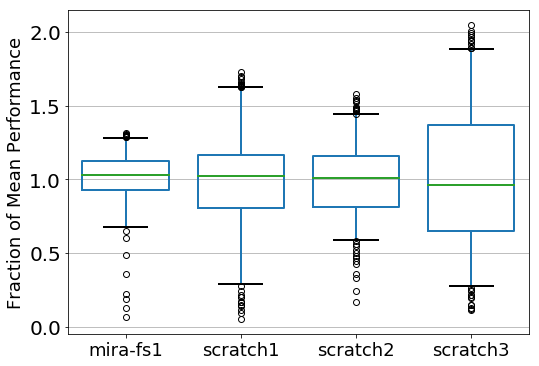
\includegraphics[width=1.0\columnwidth]{figs/perf-boxplots-per-fs.png}
\caption{TOKIO-ABC I/O performance for Edison (\texttt{scratch1},
\texttt{scratch2}, \texttt{scratch3}) and Mira (\texttt{mira-fs1}) normalized to
the mean performance of each file system.  Whiskers represent the 5th and 95th
percentiles.}
\label{fig:perf-summary-boxplots-fs}
\end{figure}

\begin{figure}[t]
\centering
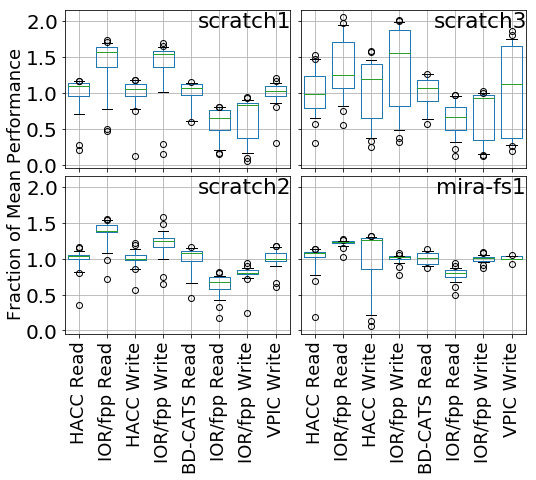
\includegraphics[width=1.0\columnwidth]{figs/perf-boxplots.png}
\caption{TOKIO-ABC I/O performance for all file systems tested grouped by test
applications and read/write mode.  Whiskers represent the 5th and 95th
percentiles.}
\label{fig:tokio-abc-perf-boxplots}
\end{figure}


%%% Glenn: the following figures are informationally sparse since I don't think
%%% we want to talk about the time dependence of performance.  I added box plots
%%% to (hopefully) more concisely show the distribution of performance.
%
% Figures \ref{fig:tokio-abc-perf-mira-fs1} and \ref{fig:tokio-abc-perf-edison-scratch1}
% show the performance of each TOKIO-ABC benchmark run on Mira's \texttt{mira-fs1} GPFS
% file system and Edison's \texttt{scratch1} Lustre file system, respectively. 
% 
% \begin{figure}[h]
% \centering
%     \subfigure[write performance]{
%         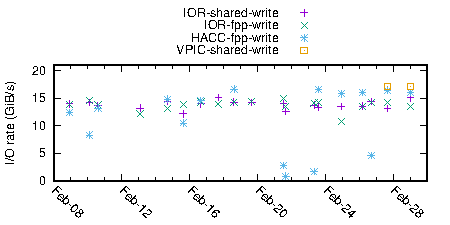
\includegraphics[width=\columnwidth]{figs/mira-fs1-write-perf.pdf}
%         \label{fig:tokio-abc-perf-mira-fs1-write}
%     }
%     \subfigure[read performance]{
%         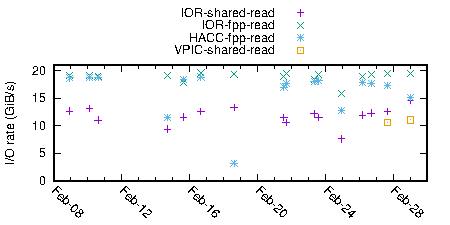
\includegraphics[width=\columnwidth]{figs/mira-fs1-read-perf.pdf}
%         \label{fig:tokio-abc-perf-mira-fs1-read}
%     }
% \caption{I/O performance for TOKIO-ABC runs on Mira's \texttt{mira-fs1} GPFS file system.}
% \label{fig:tokio-abc-perf-mira-fs1}
% \end{figure}
% 
% \begin{figure}[h]
% \centering
%     \subfigure[write performance]{
%         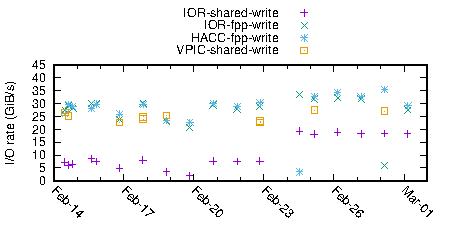
\includegraphics[width=\columnwidth]{figs/edison-scratch1-write-perf.pdf}
%         \label{fig:tokio-abc-perf-edison-scratch1-write}
%     }
%     \subfigure[read performance]{
%         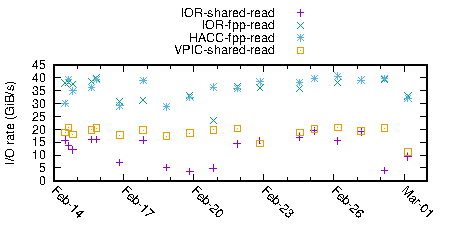
\includegraphics[width=\columnwidth]{figs/edison-scratch1-read-perf.pdf}
%         \label{fig:tokio-abc-perf-edison-scratch1-read}
%     }
% \caption{I/O performance for TOKIO-ABC runs on Edison's \texttt{scratch1} Lustre file system.}
% \label{fig:tokio-abc-perf-edison-scratch1}
% \end{figure}

Figure~\ref{fig:tokio-abc-fingerprints} shows example I/O fingerprints for the
TOKIO-ABC benchmarks on Mira and Edison.  They represent a baseline indication
of strengths, weaknesses, and susceptibility to variance for each file system.
This example shows the median performance of several workloads over time, and
performance is normalized to focus on trends rather than absolute throughput.
Whiskers indicate minimum and maximum sample values. \todo{What does this tell
us about high-level similarities/differences between Mira/GPFS and
Edison/Lustre?}

Figure~\ref{fig:tokio-abc-perf-boxplots} shows the same data (but in boxplot
format and not normalized) which suggests that the magnitude of variance in
Edison is significantly larger than the variance on Mira.  It also confirms that
shared-file I/O is more expensive than file-per-process I/O on both platforms.
\todo{What are the benefits of the fingerprint approach rather than a box plot
of the tests?  I haven't entirely thought this through so maybe the answer is
obvious.}

\begin{figure}[h]
\centering
    \subfigure[write benchmarks] {
        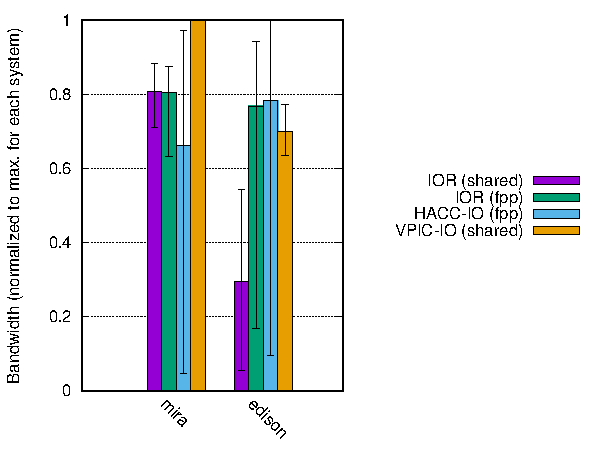
\includegraphics[width=\columnwidth]{figs/tokio-abc-write-fingerprints.pdf}
        \label{fig:tokio-abc-write-fingerprints}
    }
    \subfigure[read benchmarks] {
        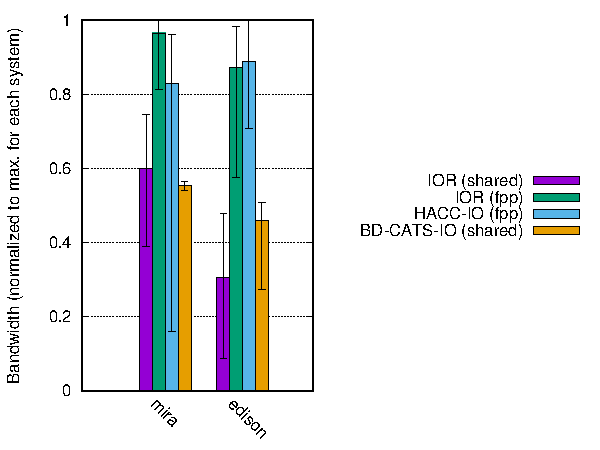
\includegraphics[width=\columnwidth]{figs/tokio-abc-read-fingerprints.pdf}
        \label{fig:tokio-abc-read-fingerprints}
    }
\caption{TOKIO-ABC I/O fingerprints for Mira and Edison.}
\label{fig:tokio-abc-fingerprints}
\end{figure}

\subsection{Discussion} \label{discussion}

This section will discuss \emph{why} we saw the behavior that we did by
correlating data sources, then make broader conclusions about the differences
between Mira and Edison results.  I envision a general approach of extracting
or calculating \emph{internal} and \emph{external} variables from the data we
have, where internal variables are measurements from components of the system
that were exclusively reserved for our jobs (e.g., all data from the compute
nodes), and external variables are those measurements from components of the
system that are shared (e.g., the file system servers).

With this premise, we then correlate these variables with performance as
measured by Darshan, essentially turning this into a smorgasbord of
multivariate analyses.  For example, Figure \ref{fig:correlate-perf-and-fstraffic}
shows the relationship between the observed benchmark performance and the
fraction of server-side traffic that can be attributed to that benchmark.
In those cases where the benchmark only represented part (e.g., less than 80
percent) of server-side traffic, benchmark performance was always poor for
some definition of poor.  Wahid suggested binning the data to reduce the
number of data points and make the correlation more obvious, or accurately
conveying the density of points that give rise to the statistically significant
correlation coefficient.

\begin{figure}[t]
\centering
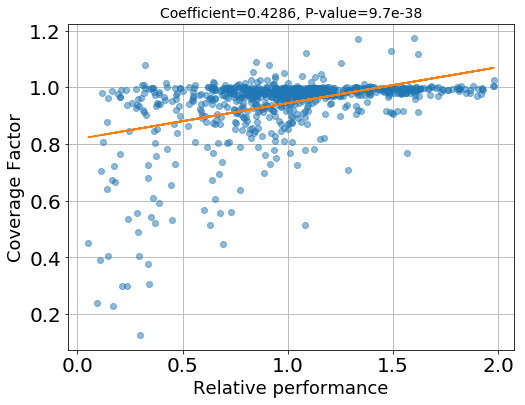
\includegraphics[width=0.8\columnwidth]{figs/edison-perf-vs-fstraffic.png}
%\vspace{-.07in}
\caption{Correlation between benchmark performance and the amount of
non-benchmark traffic occurring on the file systems on Edison}
\label{fig:correlate-perf-and-fstraffic}
\vspace{-.1in}
\end{figure}

We may also want to consider exploring if the following would be interesting:

\begin{itemize}
\item 1. Some nominally contended jobs showed good performance while others showed bad.  Why?  Correlate with metadata rates measured by backend, or CPU loads that may indicate metadata loads?  Job diameter (mostly relevant to Cray XC)?
\item 2. Can we calculate some of William's metrics during each day's jobs and correlate with that?  This should be done before the PI meeting next week.
\end{itemize}

We may also want to deep-dive into one or two specific cases of performance
degradation to root-cause them.  We have some candidates abnormally slow runs,
and we also know that VPIC-IO behaves very differently on Mira vs. Edison.
This would be a good place to showcase William's metrics and methods as well.

Once we have shown that we understand several different sources of performance
loss, we can then establish a taxonomy and enumerate how often bad I/O
performance can be attributed to each of the different causes we categorized so
that we can offer one or two specifically common sources of interference.  For
example,

\begin{itemize}
\item Sometimes metadata operations are slow (e.g., file-per-process I/O)
    \begin{itemize}
    \item Show Darshan logs showing high metadata time
    \item Show LMT MDT logs showing high background metadata or CPU rate
    \item Show GPFS NSD metadata loads?  Can we do this?
    \end{itemize}
\item Sometimes hardware goes bad
    \begin{itemize}
    \item Show Darshan logs showing bad performance at the POSIX layer (i.e., not the
    application's fault)
    \item Show Lustre OSTs that stall out, e.g, Figure~\ref{fig:example}
    \item Show slow Lustre OSTs due to failover/oversubscription (a la Darshan 3 paper)
    \item Show poorly performing GPFS NSDs
    \end{itemize}
\item Sometimes there is interference from other applications
    \begin{itemize}
    \item Show Darshan logs showing bad performance at the POSIX layer (i.e., not the
    application's fault)
    \item Show jobs with and without background LMT load
    \item Show jobs with and without background mmpmon load
    \end{itemize}
\item Sometimes tuning strategies differ across platforms
    \begin{itemize}
    \item contrast which benchmark performs best on each platform
    \item dig into why
    \item See example of how we might show this in Figure~\ref{fig:example-bar-var}
    \end{itemize}
\end{itemize}

We should refer heavily to past work (see Section \ref{related}) to make sure we
aren't reinventing anything

If we have enough data to make a statistically significant statement, we should
aim to discuss how susceptible different file systems are to these bad I/O
performance root causes to stir up controversy (GPFS is better/worse than
Lustre when facing problem X).  If we do this, we can also propose strategies
to work around these common bottlenecks.  For example, can holistic I/O
monitoring provide a feedback loop for coscheduling?

\section{Related work} \label{related}

\assign{Phil} \todo{include SIOX} Let's cite Xiaosong Ma's work in server-side
monitoring \cite{Liu2016}; her work uses server-side logs to make scheduling
recommendations based on a knowledgebase of applications and their historic
I/O requirements.  This work can improve the predictive ability of such systems
by replacing the black-box weighting parameter, $w_{i}$, with a function that
accurately captures the effects of different external interference sources for
an application.

Matthieu showed how to minimize I/O jitter~\cite{Dorier2012} (but I haven't read
this paper yet...).  More recently, Yildiz et al~\cite{Yildiz2016} performed
a systematic exploration of points of contention on an idealized system and
exposed the sensitivity of 10 GbE to various forms of interference.

Lofstead et al wrote a paper on managing I/O variability in production~
\cite{Lofstead2010} which characterizied \emph{internal interference} and
\emph{external interference} using purely client-side metrics.  They defined an
\emph{imbalance factor}, the ratio of the slowest to fastest write times, as a
means to infer the external interference, but we can precisely quantify it here
with server-side metrics.

Andrew Uselton's work on understanding I/O performance in terms of ensembles of
bursts might be relevant\cite{Uselton2010}, but his method requires heavyweight
I/O tracing to determine the statistical distribution of I/O bursts during an
application execution and, as such, as better suited to characterizing the
behavior of a specific file system as a one-time activity.

A long time ago, David Skinner and Bill Kramer wrote a paper that characterized
sources of performance variation~\cite{Skinner2005}, but it didn't really talk
about I/O in a very meaningful way.

More recently Xie et al also characterized I/O problems at Oak
Ridge\cite{Xie2012} using IOR and quantified the effects of stripe counts,
straggling writers, and shared-file I/O to target areas where middleware can
optimize I/O for applications.

Is any of the BeeGFS stuff (dynamically provisioning file systems) relevant to
interference isolation?

\section{Conclusions}

\todo{It would be great if there were some tangible artifacts from this work.
Possible examples:}
\begin{itemize}
\item open repo for benchmark configs and cron jobs so others can replicate
performance regression testing
\item anonymized data collected in study
\item new data collection tools (LMT monitoring, Lustre failover monitoring,
mmpmon monitoring, etc.)
\end{itemize}

\section{TEMPORARY: TECHNICAL TASKS}

Assumption: assignments here and in preceding text are tentative, and really
just guess at someone who can keep tabs on that activity.  Can re-assign,
delegate, pull in more people, etc.

%Assumption: although the paper as outlined will focus on Cori and Mira, we
%should actually try to do these things across Theta and Edison as well.  Four
%total platforms, and we'll see which ones are most viable for study in paper.
%
%To do:
%\begin{itemize}
%\item create git repository to store benchmarks, config files, job scripts,
%and cron configs for our set of benchmarks \assign{Shane}
%\begin{itemize}
%\item repo status: includes build scripts for hacc-io, bdcats, vpic, and ior
%\item everything works at nersc, currently testing in 96 node runs on Cori
%and Edison
%\item todo: review configurations, get ALCF configs working, settle on
%size/duration
%\end{itemize}
%
%% other benchmarks to consider later: chombo and newer version of hacc-io
%% with hdf support
%
%\item make sure that mmpmon monitoring gets deployed on Mira \assign{Phil and
%Kevin}
%\begin{itemize}
%\item timeline: currently running on Vesta, will be running on Cetus this
%Monday, will be running on Mira 2 weeks later if things look good
%\item long term plan to do same thing on Theta DVS nodes
%\end{itemize}
%
%\item coordinate LMT monitoring methods on Theta \assign{Glenn and Kevin}
%\begin{itemize}
%\item Meeting about this on Tuesday
%\end{itemize}
%
%\item enable cron jobs to run periodic jobs on ALCF machines \assign{Shane}
%\begin{itemize}
%\item Kevin working on this for Mira using Jenkins
%\item on Theta we will need to use cron with flock -n wrapper
%\end{itemize}
%
%\item enable cron jobs to run periodic jobs on NERSC machines \assign{Glenn}
%\begin{itemize}
%\item probably won't fit in backfill as is, can work on reducing time, maybe
%consider killalble queue too
%\item Glenn has been getting 4 hour runs through queue so far without much
%trouble using 96 nodes
%\item Glenn: has a master script for this already, gradually hardening, will
%add to git repo
%\item For paper: measure saturation percentage of scripts and give rationale
%for jobs of different sizes on different machines being comparable
%\item remember to plot in relative rather than absolute times in paper where
%we can, don't want people to get distracted by head to head comparison
%\end{itemize}
%
%\item create and enable cron jobs to check Lustre failover status and server
%capacity
%\begin{itemize}
%\item Glenn: already collecting this data at NERSC now
%\end{itemize}
%
%\item create and enable cron jobs to check GPFS failover status and server
%capacity
%\begin{itemize}
%\item plan to use Zach's periodic df monitoring data
%\item for failover we will have to look at logs, they are doing some
%automation already
%\end{itemize}
%
%\item start browsing existing HACC-IO data collected by Glenn to think about
%how to plot it, how to dig into details, etc. \assign{ALL}
%    
%\item contrast benchmark performance across platforms once we have stable
%daily data \assign{William and Suren}
%\end{itemize}

\begin{itemize}
    \item \textcolor{red}{ALL}: Begin analyzing TOKIO-ABC benchmark results and
    and think about how we want to correlate this with GPFS/Lustre monitoring
    data. Are there specific jobs or timeframes that we want to zoom in on
    to better understand anomalous behavior? Are there I/O trends that we
    can observe on specific systems or even across systems that would be
    interesting to the reader? This is where we want to showcase the utility
    of this framework, so we will need to find something interesting to demonstrate
    here to convince the reader. 

    \item \textcolor{red}{ALL}: begin filling in paper intro, background,
    methodology, system/benchmark descriptions, results, etc.

    \item \textcolor{red}{SHANE}: round up MMPMON data for a 2-week period
    of TOKIO-ABC runs on Mira.

    \item \textcolor{red}{GLENN}: round up LMT data for a 2-week period of
    TOKIO-ABC runs on Edison.

    \item \textcolor{red}{WILLIAM}: look at MMPMON data to determine how
    IOMiner can be extended to analyze GPFS data. 
\end{itemize}

Timeline:
\begin{itemize}
    \item \textcolor{red}{SC abstracts due March 20, 2017}
    \item \textcolor{red}{SC full submissions due March 27, 2017}
    \item Time to get moving!
\end{itemize}
%\begin{itemize}
%\item Start running periodic (daily) jobs by mid-January
%\item writing up text based on results by mid-February
%\end{itemize}
%
%Stretch goals:
%\begin{itemize}
%\item additional instrumentation sources
%\item more contributions from analysis framework perspective (i.e.,
%leveraging work from William's paper) 
%\item deploy on more platforms (either additional ALCF or NERSC systems, or
%reach out to another facility like Blue Waters)
%\end{itemize}

\bibliographystyle{IEEEtran}
\bibliography{REFERENCES}


\appendix

\section{Artifact Description}

Consider adding material here per guidance at
\url{http://sc17.supercomputing.org/2017/02/07/submitting-a-technical-paper-to-sc17-participate-in-the-sc17-reproducibility-initiative/}.


\end{document}
